%!TEX root = ../thesis.tex
Before continuing on the topic of jamming, let''s first give an introduction to the mechanics of jamming.

Jamming is a mechanism that can enable granular material to transition between solid-like and liquid-like states. These states can occur if the material is put under an external stress, figure~\ref{fig:ch:jamming:phase-transition} illustrate these states.
Much like water can shift to gas when heated and to ice when cooled. But where water is affected by thermodynamics, granular systems are not. \hl{entirely true?}
Sand, which is a granular material, may resemble a liquid as it flows through an hour glass, although the individual grains themselves are a solid structure. This is due to something called \todo{Jamming, Force chains and Fragile matter}

\begin{figure}[hb]
	\centering
  		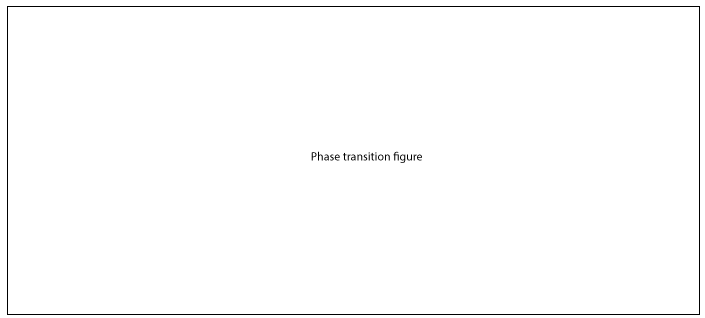
\includegraphics[width=4in]{figures/jamming/phase_transition}
	\caption[Phase transition from \textit{liquid} state to \textit{solid} state.]
   {Phase transition from \textit{liquid} state to \textit{solid} state.}
   \label{fig:ch:jamming:phase-transition}
\end{figure}

You might have noticed how some coffee packagings at the local super market are like a rigid container, see figure~\ref{fig:ch:jamming:coffee-packaging}. 
In this kind of packaging, after filling it with coffee, all excess air has been sucked out by applying a vacuum, i.e. jamming the coffee grains, and thereby making it almost rock solid. 
Also, think about a regular bean bag which exhibits some of the same properties, see figure~\ref{fig:ch:jamming:bean-bag}. 
When no force is applied to it, i.e. no one is sitting in it, it resembles the liquid-like state mentioned earlier. 
When a person then sits down in a bag air will be pressed out and the particles (most often polystyrene foam) will be pushed tightly together filling the voids  \todo{some physical term here, phase space and stuff} thereby jamming the particles making it resemble a solid ...

\begin{figure}
\centering
\begin{minipage}[t]{.5\textwidth}
  \centering
  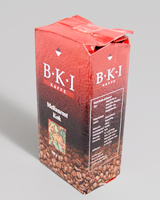
\includegraphics[width=.4\linewidth]{figures/jamming/coffee_packaging}
  \captionof{figure}{Coffee in vacuum packaging}
  \label{fig:ch:jamming:coffee-packaging}
\end{minipage}%
\begin{minipage}[t]{.5\textwidth}
  \centering
  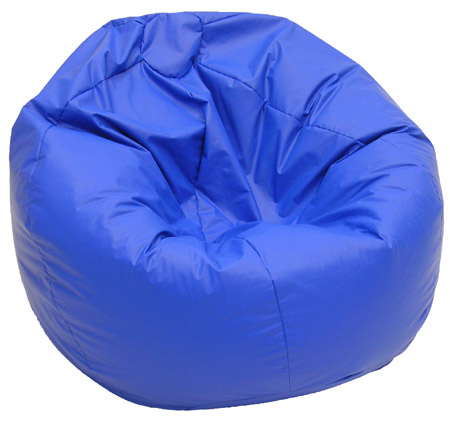
\includegraphics[width=.4\linewidth]{figures/jamming/bean_bag}
  \captionof{figure}{A bean bag}
  \label{fig:ch:jamming:bean-bag}
\end{minipage}
\end{figure}

\subsection{Particles}
\label{ch:jamming:particles}
The granular material, also called the particles, can be any material that has the physical properties that allow for jamming to occur. 
But parameters such as particle size, shape and compressibility have an impact on the jamming transition. 
This has been investigated by several researchers, e.g. \cite{cheng2012design} and \cite{steltz2010jamming}, where the stress to strain ratio \todo{explain this} of different granular materials are evaluated. 
Ground coffee (fine and coarse) and glass beads of varying size are recurring across these tests, the first being an irregular shape with a rough surface as opposed to the plain shape and smooth surface of the second, see figure~\ref{fig:ch:jamming:particles-close-up}. 
Particles of same size and with a smooth surface will tend to be more fluid-like when unjammed as they flow more freely. 
Irregular particles with rough surfaces will create more friction between the particles thus being less fluid-like in the unjammed state.

The conclusion is that the choice of granular material is very much dependent on the application in question. 

\begin{figure}
\centering
\begin{subfigure}{.5\textwidth}
  \centering
  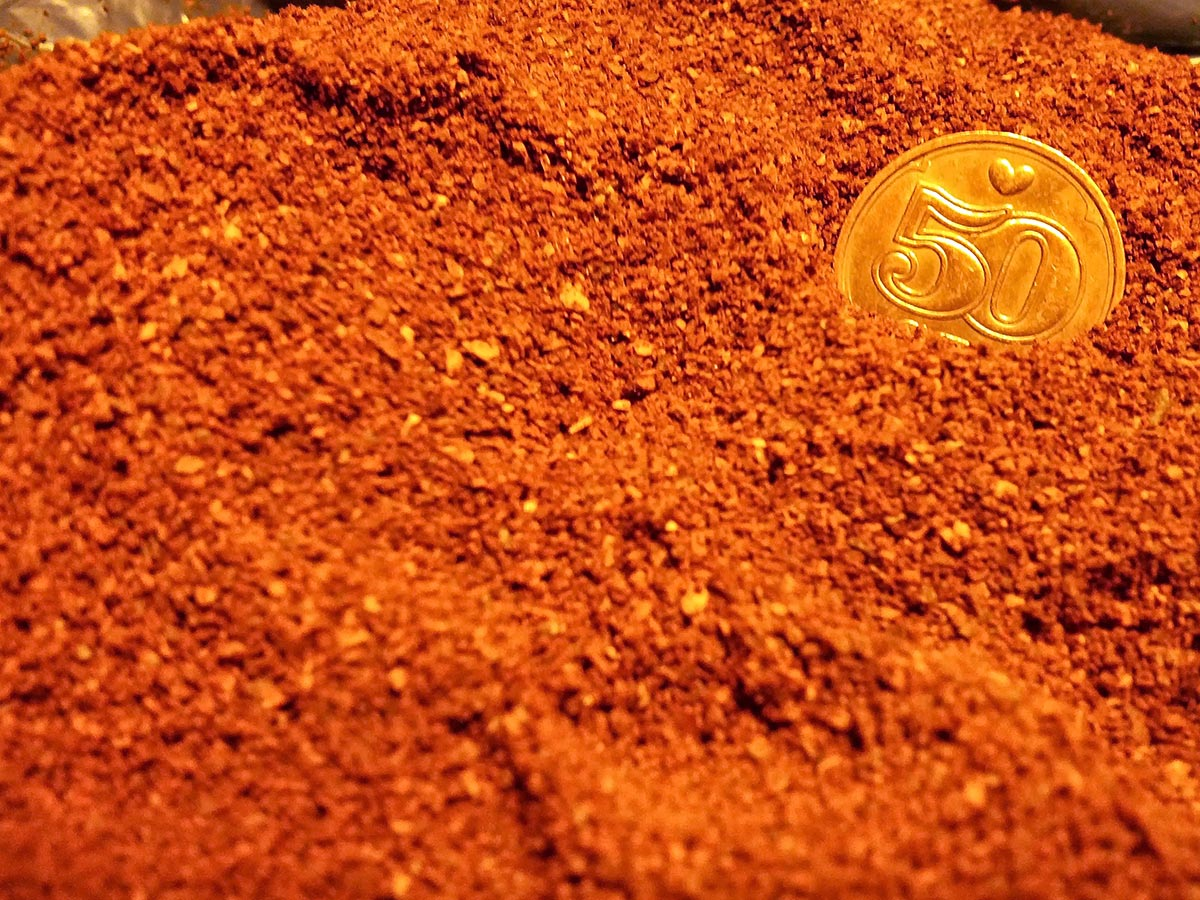
\includegraphics[width=.4\linewidth]{figures/jamming/coffee-grains}
  \caption{Grounded coffee}
  \label{fig:sub1}
\end{subfigure}%
\begin{subfigure}{.5\textwidth}
  \centering
  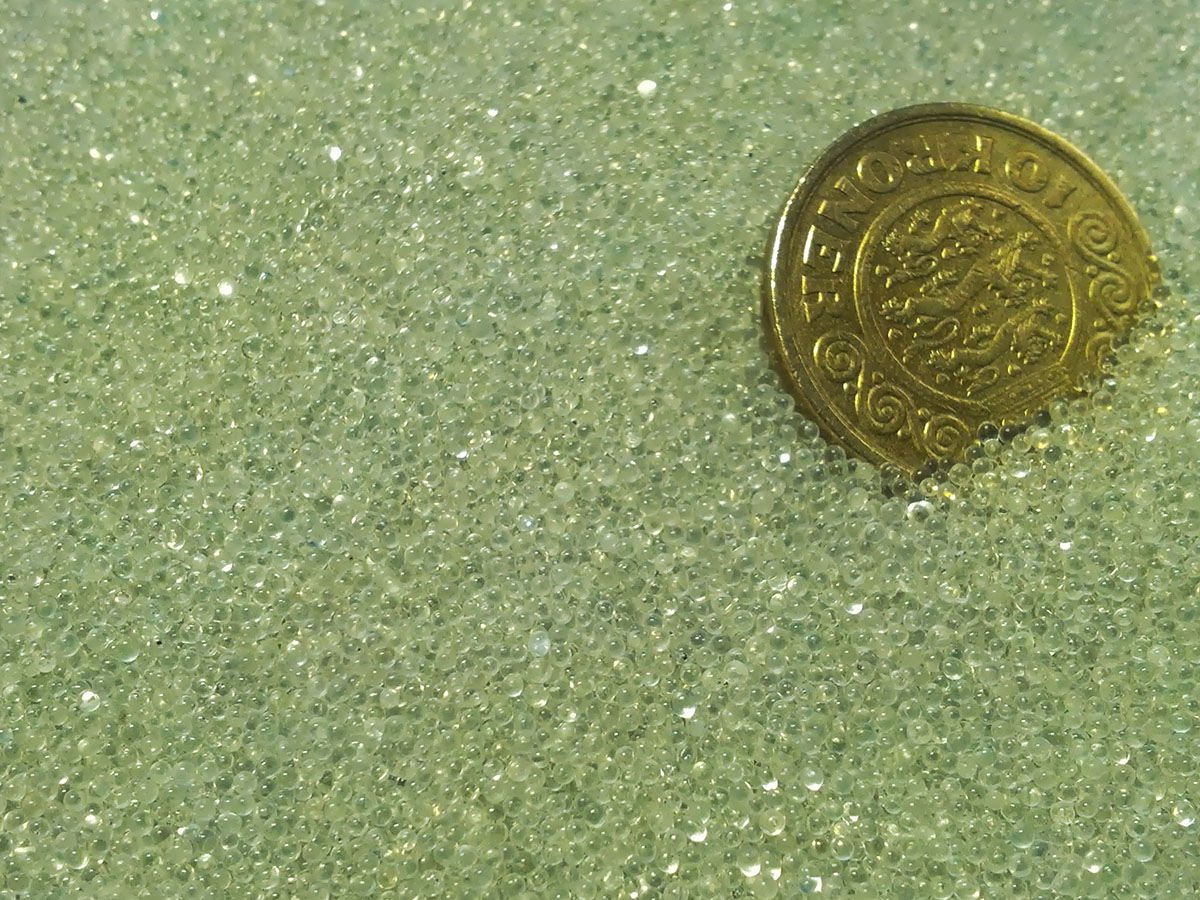
\includegraphics[width=.4\linewidth]{figures/jamming/glass-beads}
  \caption{Glass beads}
  \label{fig:sub2}
\end{subfigure}
\caption{A microscopic view of different granular material.}
\label{fig:ch:jamming:particles-close-up}
\end{figure}

\todo{research in particle parameters in other\\ disciplines such as robotics.}

\begin{itemize}
	\item http://en.wikipedia.org/wiki/Jamming\_(physics)
	\item http://www.nature.com/nphys/journal/v3/n4/full/nphys580.html
	\item http://www.nature.com/nature/journal/v411/n6839/full/411772a0.html
\end{itemize}

\subsection{The technique}
\label{ch:jamming:technique}


\subsubsection{Pneumatic jamming}

In the pneumatic approach a gas, for example air, is used as a means for actuation, see figure~\ref{fig:ch:jamming:jamming-basics}.
The gas is enclosed together with the granular material within a flexible and air tight container, for example rubber latex. 
A filter prevents the granular material from escaping the container and a valve upholds the pressure.
An external vacuum pump can then suck out the air of the container, creating a negative pressure \todo{or vacuum} inside, which results in the transition to a solid-like form. 
The speed of this transition of course depends on the suction power of the pump.
When the vacuum is released the form will gradually transition back to the liquid state. 
\todo{It is not just a two-state system}
In this way it is possible for instance to deform a jammable object by hand while in the liquid state and then apply the vacuum and make the deformed object solid - in a sense the form is \emph{saved} as long as the vacuum is maintained.

\begin{figure}[hb]
	\centering
  		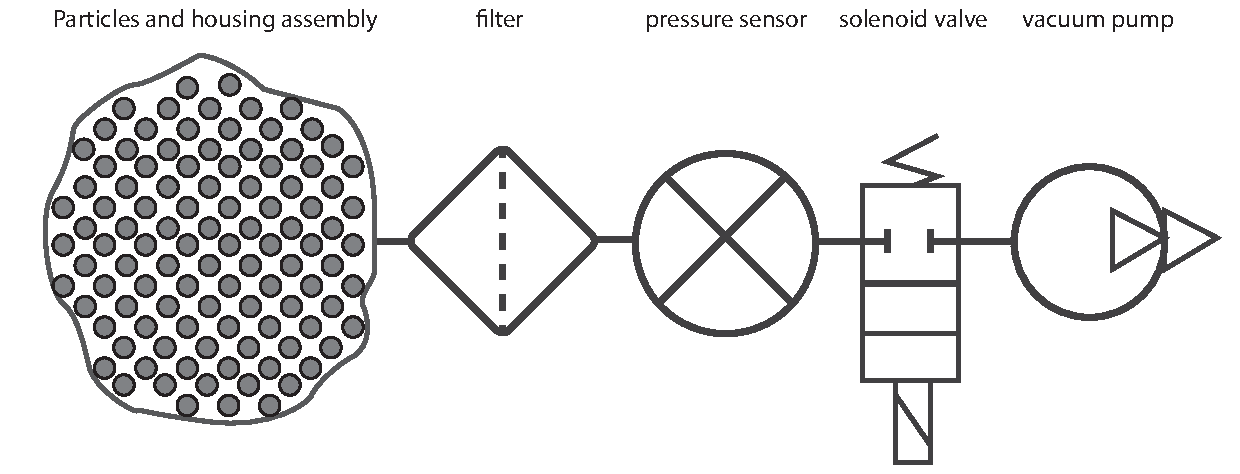
\includegraphics[width=4in]{figures/jamming/jamming-basics}
	\caption[A basic pneumatic jamming system.]
   {A basic pneumatic jamming system.}
   \label{fig:ch:jamming:jamming-basics}
\end{figure}

\subsubsection{Hydraulic actuation}
Hydraulic jamming works basically in the same way as pneumatic jamming but with liquid instead of gas as a means for actuation. 
\todo{more to come}